\chapter{Implementation and Testing}

\section{Survey Statistics}

With some of the preliminary respondents answering the survey questions, there was immediately an incredible amount of points to learn from. Early responses lead to a need for a set of patches to be made after the first day and the reasoning behind this is discussed in section 5.2. While there was not originally any plans to make any major code changes after deployment, there was an incredible demand to make the system easier to use moving forward and help respondents be able to complete the survey rather than creating biased responses.
\newline
\newline
With the early responses however, there were also a great deal of positive points learned. Looking at the early responses, a few trends started to emerge showing some of the lacking features but also how much of a demand there is for this service to be provided by the university. Users were early on prompted if they used a mobile device at first to access the website and then asked if they would have preferred this. The reason they were asked this was the survey was often shared via a text message, thus leading to users attempting to use their mobile device. The reasoning behind this decision was to see how users approached the system and if there would be a realised demand for mobile support on the site or not. Responses are then shown in figure \ref{fig:mobile_support}.

\pagebreak
\begin{figure}[ht]
\centering
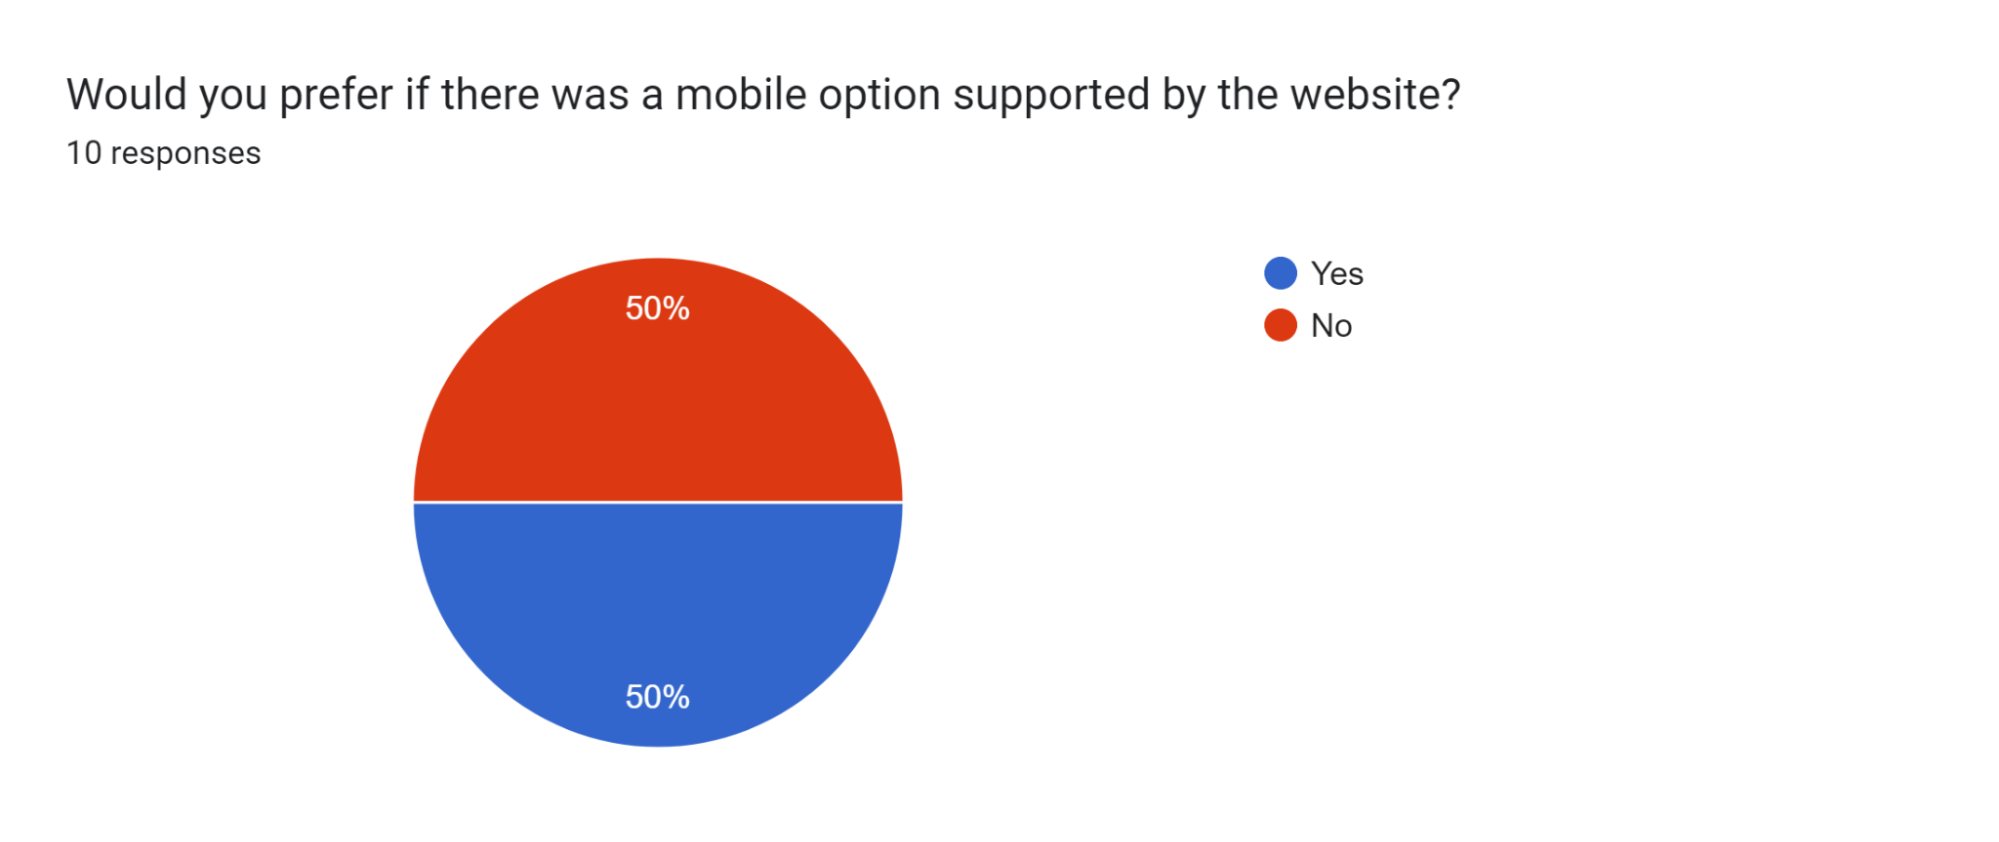
\includegraphics[width=15cm]{myReport/images/mobile_option.png}
\caption{Response demand for a mobile application version}
\label{fig:mobile_support}
\end{figure}

After seeing results for Figure \ref{fig:mobile_support}, it was incredibly surprising to see that most users prefer to simply have a desktop version available to submit an extenuating form. With over 70\% of respondents claiming that they do not desire to have a mobile version even offered, it was very clear that there was little demand for such an application.

\begin{figure}[H]
\centering
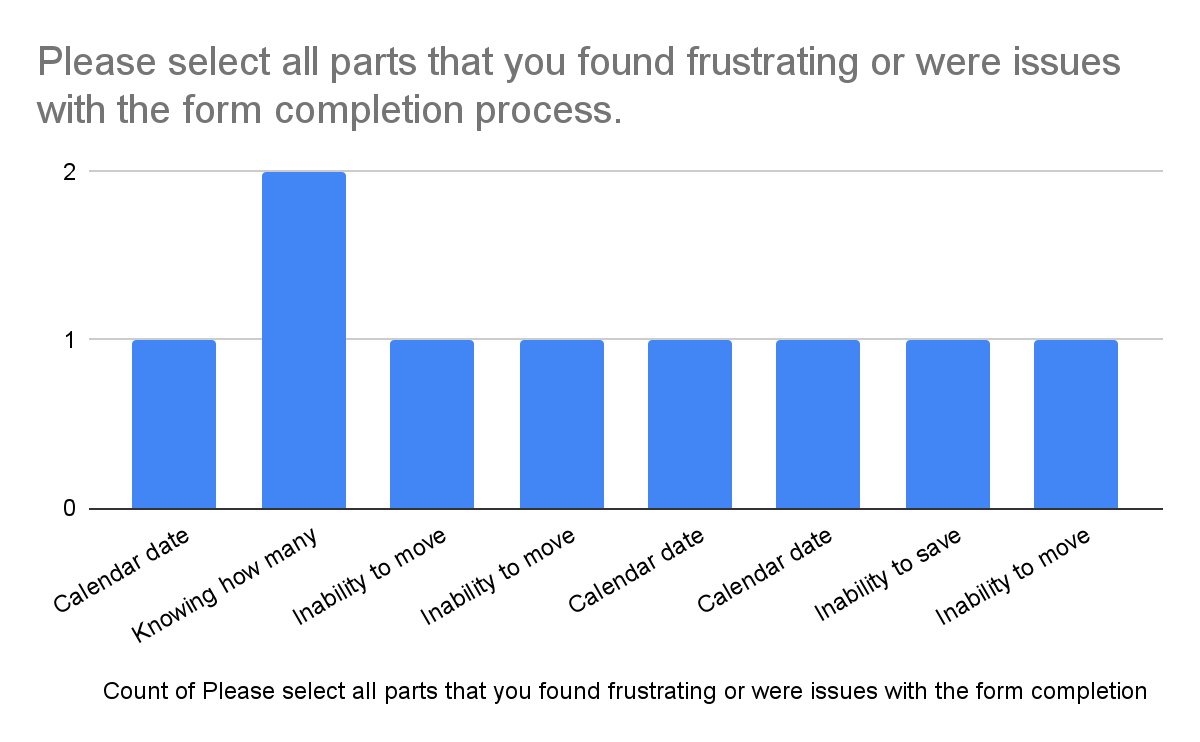
\includegraphics[width=15cm]{myReport/images/image8.png}
\caption{Common frustrations users felt while using the site}
\label{fig:user_furstrations}
\end{figure}

Of the options available to users for what was found difficult to use, it was clear that the most common frustration was knowing how many pages were left in a form. This was further compounded by a user responding “You can see everything you need to fill out ahead of time all at once” as a requested feature. 
\newline
\newline
With as many issues as users faced however, there was a 100\% response rate of users indicating that a system like the demo was vastly superior to the current implementation of using a word document. This proof of concept shows that the paper system causes more headaches for both staff and students alike and the resource cost to further develop this demo into a deployed system would be worthwhile. This is further demonstrated by Figure \ref{fig:friendliness}.

\begin{figure}[H]
\centering
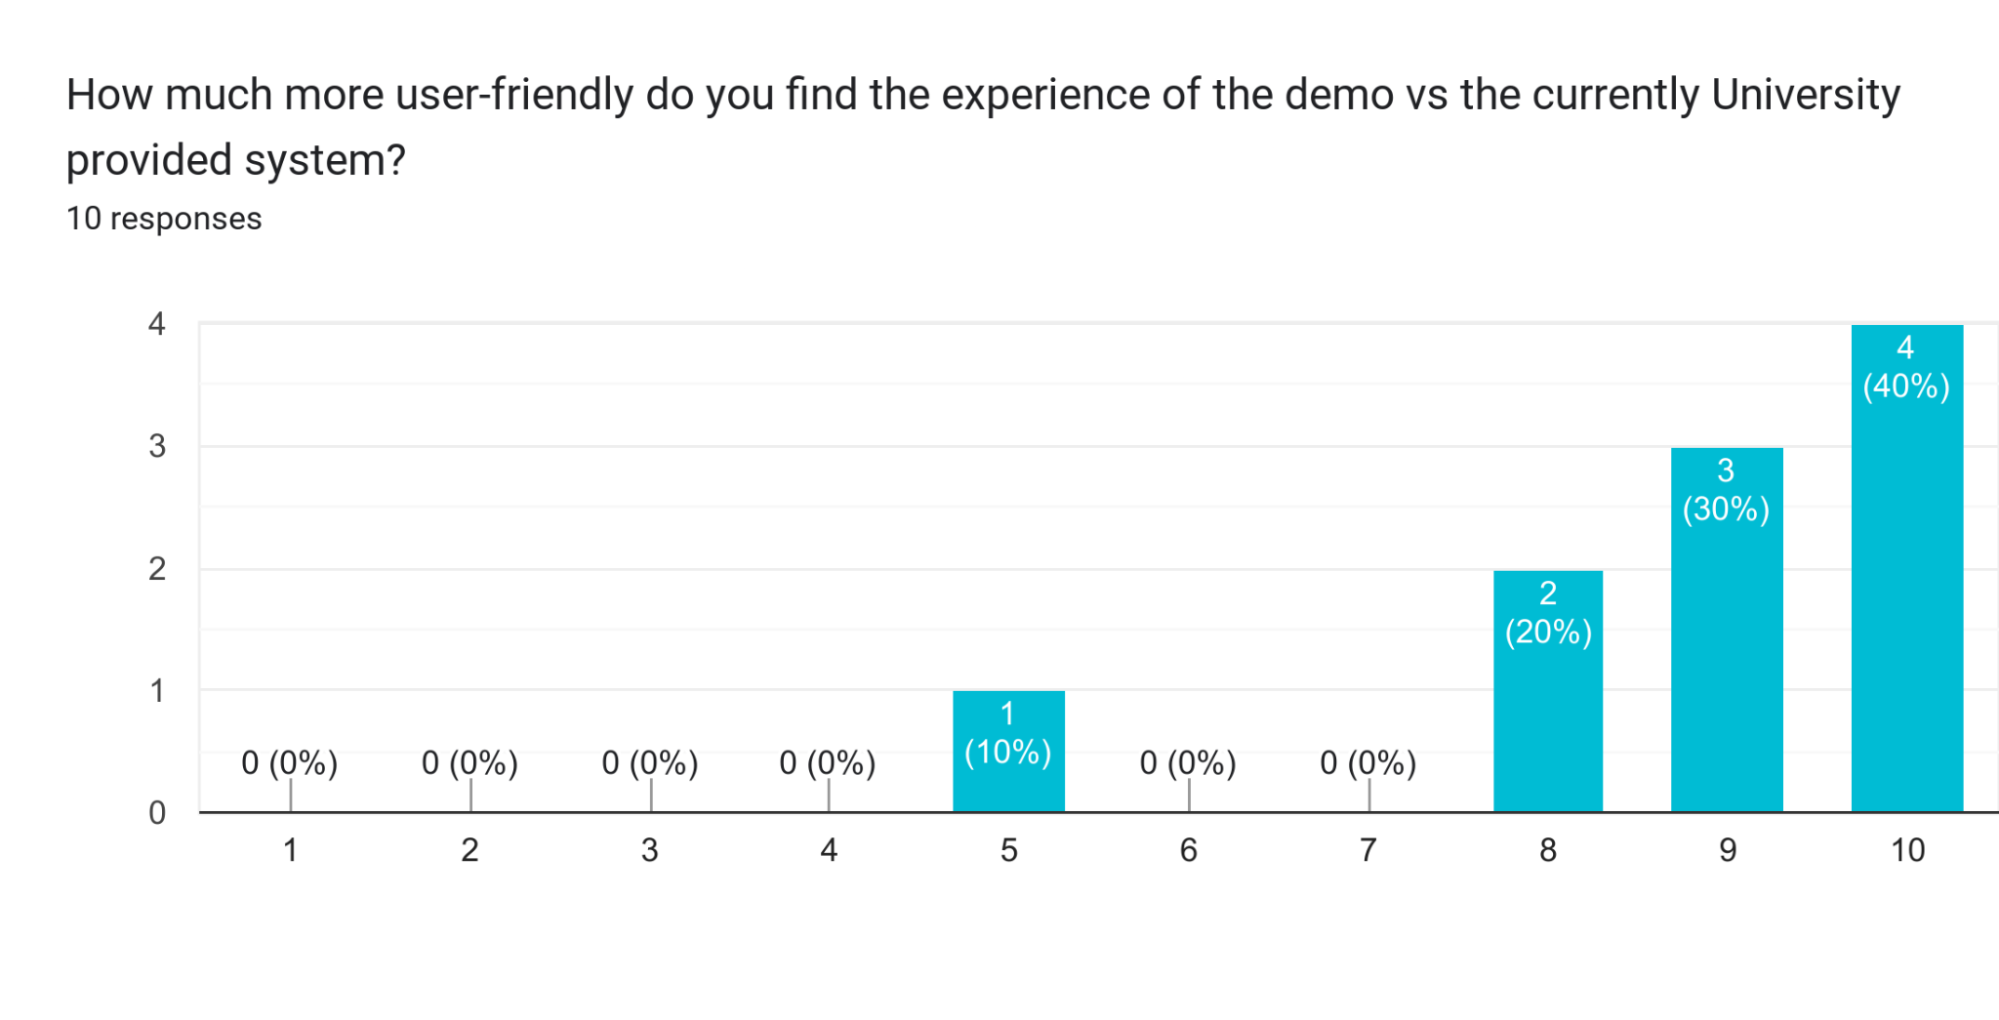
\includegraphics[width=15cm]{myReport/images/image7.png}
\caption{Range of user friendliness level}
\label{fig:friendliness}
\end{figure}

In Figure \ref{fig:friendliness}, a range of user friendliness level from 1 being biased towards the university paper system and 10 being the deployed demo being more user friendly instead was asked of users. A 10 denotes pure preference towards the provided demo and there was a clear trends towards this.

\section{Day One Patch}

After reviewing the early responses from users, many found it difficult to create simple accounts given there was little information given to the user other than that they had provided invalid information. This included not providing a valid email address or attempting to use a student ID number that was already used by another account. This led to issues that were not realised at the time of development. 
\newline
\newline
In order to make the experience at least usable to users so that they did not give up and not fill out the survey, a patch was created to give the user far more insight into why they couldn’t create an account. This includes protection in the field for student IDs which must be 9 digits long as well as email validation using a regular expression. The chosen regular expression in this hot-fix was the fully RFC 822 compliant regex as it is both an international standard now as well as it did not require much work on development to implement.
\newline
\newline
The original system would simply notify a user that the back-end responded with a 400 if something went wrong. While this worked in development just fine, it was found to be incredibly confusing for users and resulting in not understanding what was going wrong. By implementing these safeguards after the first day of testing, it made the rest of the respondents not want to stop using the system early on. While there is a fear of skewing the rest of the responses to be far more positive with these changes, it was weighed that it instead makes it easier for non-technical users to understand and use the demo. 

\section{Technical Responses}

When working with respondents, users were also prompted for their understanding and usages of both back-end and front-end frameworks that they have used in the past. The goal of asking these questions was to ascertain whether the demo would be considered technically difficult based on the chosen design patterns and if there were any critical flaws in design that jumped out to any programmers. This would further aid in the day one patch that was done as it would show what kind of stresses the demo would have to endure. The responses can be seen in Figures \ref{fig:backend_frameworks} and \ref{fig:frontend_frameworks}.

\pagebreak
\begin{figure}[ht]
  \begin{subfigure}{\linewidth}
    \centering
    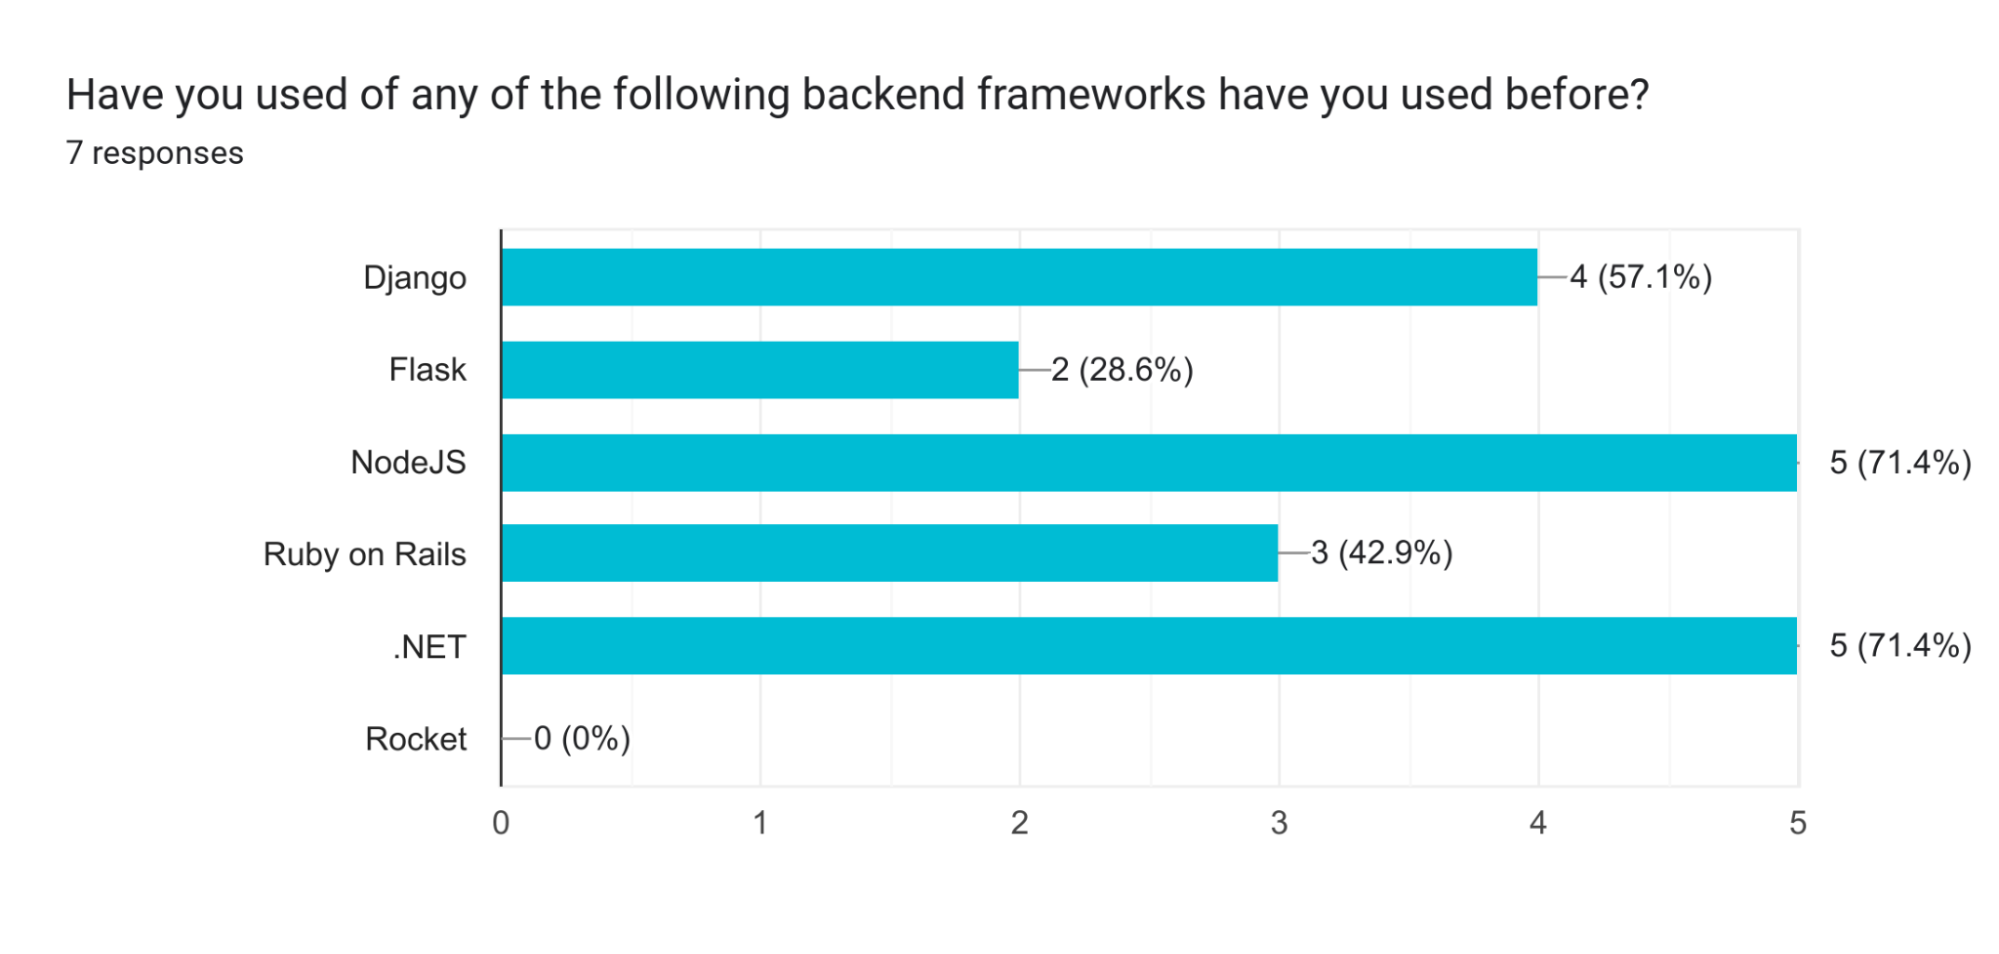
\includegraphics[width=0.8\linewidth]{myReport/images/image6.png}
    \caption{Number of users who have used any of the listed back-end frameworks before}
    \label{fig:backend_frameworks}
  \end{subfigure}
  
  \begin{subfigure}{\linewidth}
    \centering
    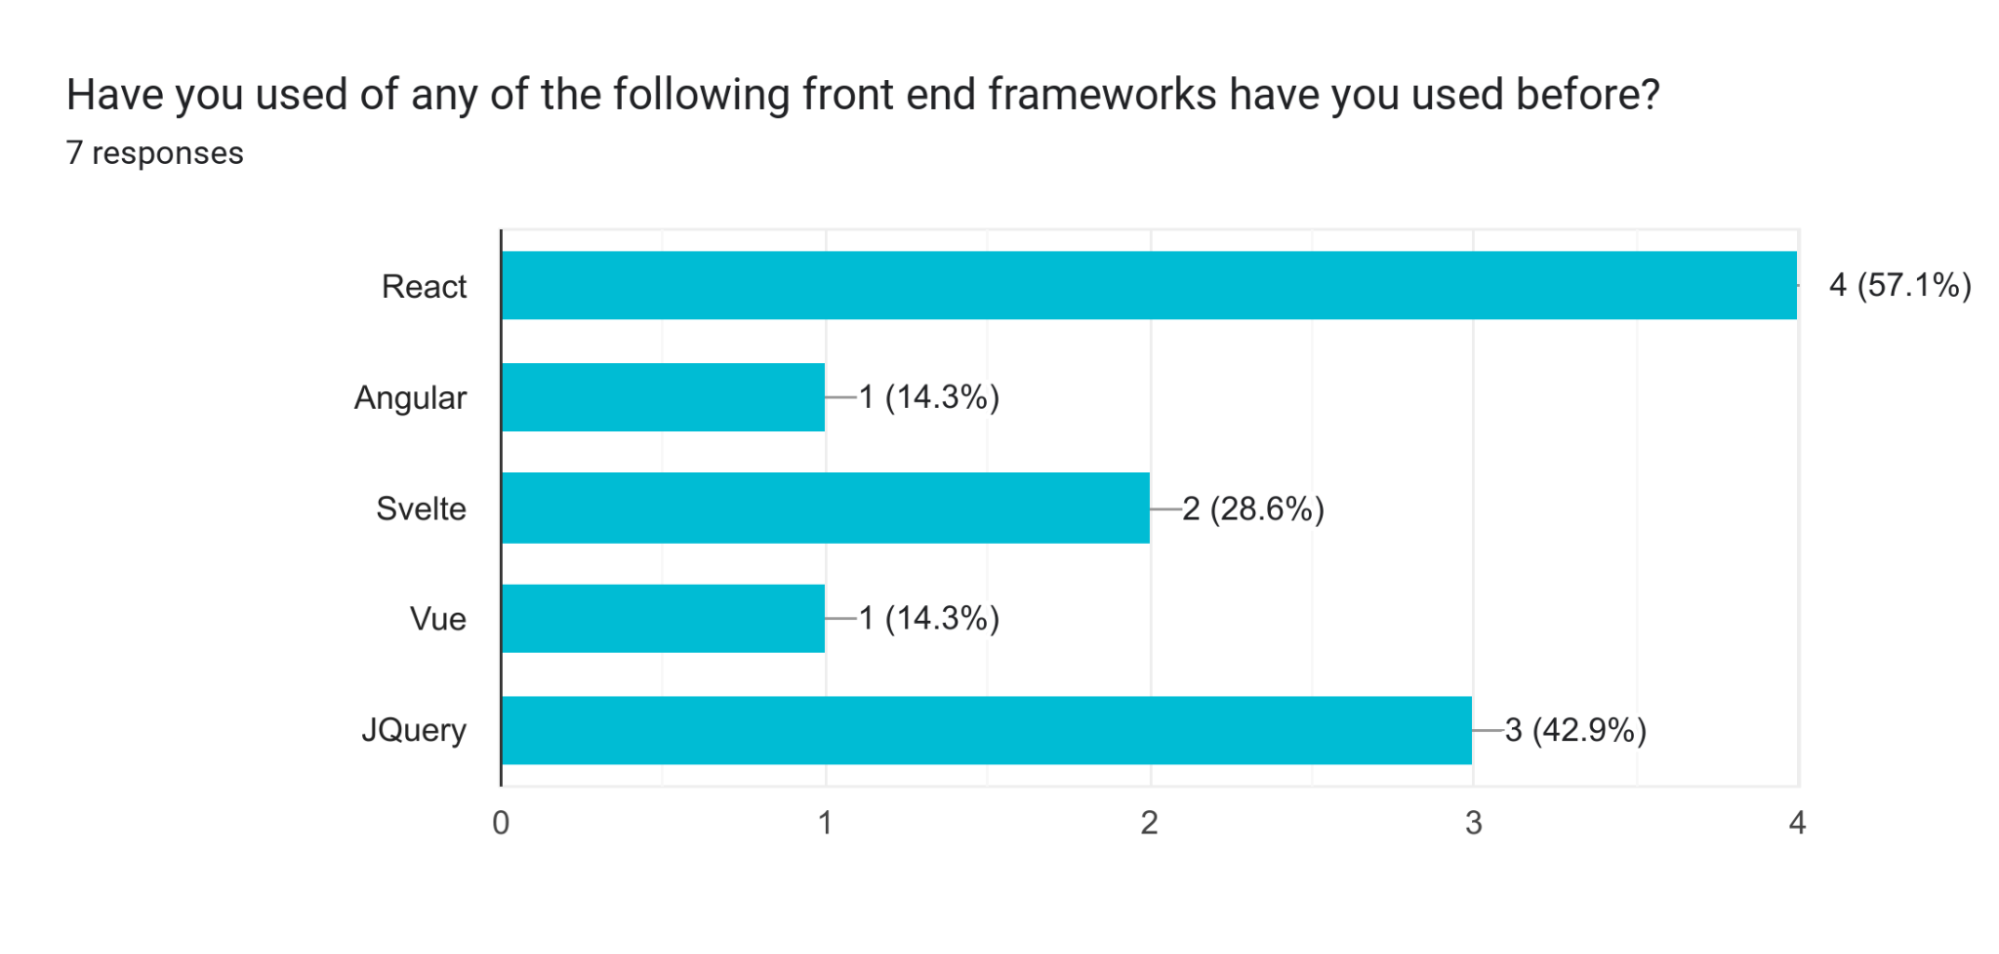
\includegraphics[width=0.8\linewidth]{myReport/images/image9.png}
    \caption{Number of users who have used any of the listed front-end frameworks before}
    \label{fig:frontend_frameworks}
  \end{subfigure}
\end{figure}

\section{Server Up-time}

By moving over to a deployed version of the web app, this established that all future alterations and modifications to the service would necessitate database migrations moving forward to preserve user data. This included regular checks from the development team’s time to ensure that users could respond whenever they want to the survey on their own time and also checking logs for any irregularities, hiccups, or potential memory leaks within the software itself.
\newline
\newline
There was a reported incident of an AWS EC2 outage in the middle of the project that did cause a slight issue for the development team during the deployment of the project. This was halfway through the survey time frame and did require a little bit of looking before seeing that the virtual machine had restarted itself and redeployed everything correctly. This did cause a bit of stress from a development standpoint as outages are the worst possible scenario for an application such as this, but fortunately no users were accessing the website during the outage and the problems did resolve themselves after AWS had everything restarted within 15 minutes.
\newline
\newline
One of the issues some users would have is browsers would block access to the website on occasion as an SSL certificate was not issued. While the demo did not quite need one as the domain name was temporary and only used for the purposes of research, it did cause potential problems with certain machines accessing the site. In a live production build that is not a demo, this would never be an issue as the university would be able to utilise the official Sheffield SSL certificate, but this is a point to consider for future survey responses and access for users.